%%%%%%%%%%%%%%%%%%%%%%%%%%%%%%%%%%%%%%%%%%%%%%%%%%%%%%%%%%%%%%%%%%%%%%%%%%%%
% AGUJournalTemplate.tex: this template file is for articles formatted with LaTeX
%
% This file includes commands and instructions
% given in the order necessary to produce a final output that will
% satisfy AGU requirements, including customized APA reference formatting.
%
% You may copy this file and give it your
% article name, and enter your text.
%
% guidelines and troubleshooting are here: 

%% To submit your paper:
% \documentclass[draft]{agujournal2019}
% \usepackage{url} %this package should fix any errors with URLs in refs.
% \usepackage{lineno}
% \usepackage{booktabs}
% \usepackage{graphicx}
% \usepackage{subcaption}
% \usepackage{float}

% % \usepackage[inline]{trackchanges} %for better track changes. finalnew option will compile document with changes incorporated.
% \usepackage{soul}
% \linenumbers
%%%%%%%
% As of 2018 we recommend use of the TrackChanges package to mark revisions.
% The trackchanges package adds five new LaTeX commands:
%
%  \note[editor]{The note}
%  \annote[editor]{Text to annotate}{The note}
%  \add[editor]{Text to add}
%  \remove[editor]{Text to remove}
%  \change[editor]{Text to remove}{Text to add}
%
% complete documentation is here: http://trackchanges.sourceforge.net/
%%%%%%%

% \draftfalse

%% Enter journal name below.
%% Choose from this list of Journals:
%
% JGR: Atmospheres
% JGR: Biogeosciences
% JGR: Earth Surface
% JGR: Oceans
% JGR: Planets
% JGR: Solid Earth
% JGR: Space Physics
% Global Biogeochemical Cycles
% Geophysical Research Letters
% Paleoceanography and Paleoclimatology
% Radio Science
% Reviews of Geophysics
% Tectonics
% Space Weather
% Water Resources Research
% Geochemistry, Geophysics, Geosystems
% Journal of Advances in Modeling Earth Systems (JAMES)
% Earth's Future
% Earth and Space Science
% Geohealth
%
% ie, \journalname{Water Resources Research}

% \journalname{Journal of Advances in Modeling Earth Systems (JAMES)}


% \begin{document}

%%%%%%%%%%%%%%%%%%%%%%%%%%%%%%%%%%%%%%%%%%%%%%%
%  TITLE
%
% (A title should be specific, informative, and brief. Use
% abbreviations only if they are defined in the abstract. Titles that
% start with general keywords then specific terms are optimized in
% searches)
%
%%%%%%%%%%%%%%%%%%%%%%%%%%%%%%%%%%%%%%%%%%%%%%%

% Example: \title{This is a test title}

% \title{Training neural mapping schemes for satellite altimetry with ocean model data}


% \authors{Q. Febvre\affil{1}, J. Le Sommer\affil{2}, C. Ubelmann\affil{3}, R. Fablet\affil{1}}

% \affiliation{1}{IMT Atlantique, Lab-STICC, Brest, France}
% \affiliation{2}{Université Grenoble Alpes, CNRS, IRD, Grenoble, France}
% \affiliation{3}{Datlas, Grenoble, France}

% \correspondingauthor{Quentin Febvre}{quentin.febvre@imt-atlantique.fr}



% \begin{keypoints}
% \item We propose a simulation-based training approach for the neural mapping of real satellite-derived observations.
% \item Simulation-trained neural schemes significantly outperform the operational mapping of real altimetry data for a Gulf Stream case-study.
% \item More realistic simulation datasets improve the performance of the trained neural mapping both quantitatively and qualitatively. 

% \end{keypoints}

\begin{bibunit}[IEEEtran.bst]

\clearemptydoublepage
\chapter{Training neural mapping schemes for satellite altimetry with ocean model data}

\begin{abstract}
  The absence of reference data, which defines the expected model outputs, poses a challenge when training machine learning models with ocean observations. Here, we put forward the idea that leveraging both simulated observations and ocean quantities for learning purposes provides a powerful method to develop real-world applications.
  For example, we focus here on the problem of satellite altimetry interpolation which consist in reconstructing the dynamic field of sea surface height (SSH) from satellite observations that have a high rate of missing data and irregular sampling. Data-driven models have been successfully demonstrated for this task in supervised settings using an observation simulated system experiment (OSSE), i.e. with a simulated SSH field as learning target and pseudo-observations as inputs.
  However the learning paradigm used in those demonstrations can not be trivially transferred to real altimetry observations by lack of knowledge of the true SSH field.
  We ask here if and under what condition the knowledge extracted from synthetic data transfers to real observations. We study the impact of the ocean run resolution, observation data reanalysis and of explicit tide modeling on training an interpolator over the Gulfstream region. We find that the different datasets reliably offers better performance than the current operational product DUACS when evaluated on real altimetry data. Additionally, a more realistic ocean simulation through higher resolution or model reanalysis has been shown to be significant for achieving better reconstruction performance on our test case. Our best model improves the longitudinal scale resolved from 151 kilometers for DUACS to 98 kilometers and improves the root mean squared error (RMSE) by 23\%.
  We believe that this work opens interesting perspectives for developing synergies between ocean modeling and operational product development by leveraging learning based approaches.

\end{abstract}

\section*{Plain Language Summary}

% https://www.agu.org/Share-and-Advocate/Share/Community/Plain-language-summary
In order for an artificial intelligence to learn, one need to describe a task using data and an evaluation procedure. For example, to train a model to recognize trees, one need pictures of trees and the labels of the type of tree in the pictures to evaluate and train the model.
For some problems we have access to a lot of data but cannot easily train a model because we can't easily tell how good it's performing. This happens in ocean science where a lot of instruments gather observation data but it's not always easy to compute what the model should be trained for.
Here we look at a specific task which is to construct images related to the ocean surface currents from what satellites can see. The satellite data we're using can be seen as an image of the ocean surface with a lot of missing data (~95\% of missing pixels for a given day), and we would like to train an artificial intelligence to find the values of the missing pixels.
As described before, when our model fills the gaps a certain way, we cannot easily say how good is the reconstruction because we don't know the full image. It is therefore challenging to train such an artificial intelligence using only the satellite data.
However, scientists know a lot about the ocean, how the currents behave and they're able to simulate fake oceans in big computers. For these fake oceans, we do have access to the gap-free image, so we can train A.I. models by first hiding some pixels and checking if the model fill the gaps with the correct values.
In this paper we explore if A.I.s trained on fake oceans are useful for the real ocean and study what is the best fake ocean for training an A.I.
We show that today's fake oceans work well for training an A.I. on this specific task and that the best way to obtain a great A.I. is to use a fake ocean that has been simulated with a higher resolution!


\section{Introduction}


% ML pour traitement de données satellite, bcp d'applications recentes 

% en particulier tache de gap-filling et cartoigraphie 

% un bon exemple altimétrie, methodes expertes et methodes methodes basées données. 

%--- [difficulté : suprenante, pas vraiment assez de données pour entrainer algo complexe (millions partame) [en fait non]]

% algo basé donnée : modele parametrique (calibration faible nombre de params : MIOST, DYNMOST), algo issue du DL (grnd nombre de param, NN expressif, peu d'hypothese)

% algo DL, besoin de bcp de données, en prqtique, peuvent entrainée sur données modeles. ex papier de SEATTLE. (emergence : modele numerique pour ca.) 

% question comment se fait le tranfert, sous quelle condition un lodele est-il bon poru entrainer algo pour tache donées reel. 

% Dans cet article, on demontre que modele peut marcher, cas particuler altimétrie, influence de la donnée d'entrée 

% le plan de l'artle, c'est ca 



  Satellite altimeters have brought a great leap forward in the observation of sea surface height on a global scale since the 80's. They have greatly contributed to the monitoring and understanding of key processes such as the rise of the mean ocean level due to rising temperature and the role of mesoscale dynamics.
  
  The retrieval of mesoscale-to-submesoscale sea surface dynamics for horizontal scales smaller than 150 km however remains a challenge for operational systems based on optimal interpolation \cite{taburetDUACSDT2018252019} and data assimilation \cite{jean-michelCopernicusGlobal122021} schemes. This has motivated a wealth of research to develop novel mapping schemes \cite{ballarottaDynamicMappingAlongTrack2020,ubelmannReconstructingOceanSurface2021,guillouMappingAltimetryForthcoming2021}.

  In this context, data-driven and learning-based approaches \cite{alveraazcarateReconstructionIncompleteOceanographic2005,barthDINCAEMultivariateConvolutional2022,lguensatAnalogDataAssimilation2017,fabletENDTOENDPHYSICSINFORMEDREPRESENTATION2021,martinSynthesizingSeaSurface2023} appear as appealing alternatives to make the most of the available simulation and observation datasets. Especially, Observing System Simulation Experiments (OSSE) have stressed the potential of the supervised learning of neural schemes for the mapping of satellite-derived altimetry data \cite{fabletENDTOENDPHYSICSINFORMEDREPRESENTATION2021,beauchamp4DVarNetSSHEndtoendLearning2023}. 
  
  Their applicability to real datasets has yet to be assessed and recent studies have rather explored unsupervised learning strategies from real gappy multi-year altimetry datasets \cite{martinSynthesizingSeaSurface2023}. Despite promising results, these schemes do not reach the relative improvement of the operational processing suggested by OSSE-based studies.
  
Here, we go beyond the exploitation of OSSE as benchmarking-only testbeds. We explore their use for the training of neural mapping schemes which we apply to real altimetry dataset. Through numerical experiments on a Gulf Stream case-study for 2003-2005 4-nadir altimeter constellation, our key contributions are as follows:  

    \begin{itemize}
    \item{We demonstrate the relevance of the supervised OSSE-based learning of neural mapping schemes for the space-time interpolation of real nadir altimetry data;}
    \item{We benchmark the proposed approach with state-of-the-art operational products as well as neural schemes trained from real altimetry datasets;}    
    \item{We benchmark neural schemes trained with the proposed OSSE-based strategy using different simulation datasets and we assess the impact of the characteristics of these datasets on the mapping performance.}
%    Demonstrate numerically that today's numerical simulations of the ocean are a valuable resource for training machine learning models to be applied on real data, with added benefit of more realistic synthetic data}
    \end{itemize}
To ensure the reproducibility of our results, our code is made available through an open source license along with the considered datasets and the trained models.

    
The content of this paper is organized in the following manner. Section \ref{sec:background} offers background information on related work, Section \ref{sec:method} presents our method, Section \ref{sec:results} reports our numerical experiments, and Section \ref{sec:discussion} elaborates on our main contributions.



\section{Background}
\label{sec:background}
\subsection{Satellite altimetry gridded products}
\label{ssec:interpolation}
The mapping of altimetry data to produce gridded products is a necessary step to observe surface dynamics since geostrophic currents depend on the SSH gradients which cannot be directly computed from one dimensional altimetry data. We can distinguish three categories of approaches to produce such maps. 

Data assimilation products that use large ocean models such as the GLORYS12 reanalysis \cite{jean-michelCopernicusGlobal122021}. These products leverage the full expressiveness of state of the art ocean models and aims at generating trajectories close to observed quantities through data assimilation methods such as Kalman filters and four dimensional variational data assimilation (4DVAR)\cite{carrassiDataAssimilationGeosciences2018}. In the case of the GLORYS12 reanalysis, alitmetry data was assimilated as well as ocean salinity, surface temperature and sea-ice concentration observations.

Then, observation products that are made with little dynamical assumptions such as optimal-interpolation-based product DUACS \cite{taburetDUACSDT2018252019} or methods that involve simplified quasi-geostrophic dynamics to guide the interpolation scheme. \cite{guillouMappingAltimetryForthcoming2021},\cite{ballarottaDynamicMappingAlongTrack2020}

Finally in recent years, data-driven interpolation schemes including neural network based approaches recently gained momentum \cite{alveraazcarateReconstructionIncompleteOceanographic2005,fabletENDTOENDPHYSICSINFORMEDREPRESENTATION2021,ubelmannReconstructingOceanSurface2021}.



\subsection{Ocean Modeling and OSSE}
\label{ssec:oceanmodeling}
Efforts in modeling and simulating ocean physics have been essentials for better understanding the processes involved in the earth system and being able to project future behaviours \cite{bernardImpactPartialSteps2006,ajayiSpatialTemporalVariability2020}. 
High resolution simulations used in Observing System Simulation Experiments (OSSE) also provide a great test-bed for developing and evaluating new ways observing the ocean.
Access to the numerical model outputs enables the computation of interpretable metrics directly on the quantities of interest. This can be challenging when working with observation data which need to go through a series of processing steps to estimate before being interpretable.
For example, in the case of the recently launched SWOT mission, a novel instrument has been deployed and the calibration methods were developed and evaluated using ocean and instrument simulations \cite{dibarboureDataDrivenCalibrationAlgorithm2022}.
Similarly, the development of new methods for interpolating altimetry tracks and SWOT data such as the BFN-QG and 4DVarNet were also first demonstrated in OSSE setups \cite{guillouMappingAltimetryForthcoming2021,fabletENDTOENDPHYSICSINFORMEDREPRESENTATION2021}. 



\subsection{Tackling the lack of annotated data}
\label{ssec:transferlearning}
In OSSE setups, learning based mapping schemes can be trained on reconstructing the model outputs considered as the ground truth during evaluation. However such training procedures cannot be trivially transferred  when transitioning to Observing System Experiments (OSE) by lack of knowledge of the ocean state.
Applied machine learning practitioners often face the challenge of limited annotated data when training supervised learning schemes since creating large annotated datasets for a given task can be expensive or infeasible.
Prior research efforts have tackled this issue by either leveraging existing related annotated datasets such as the ImageNet\cite{dengImageNetLargescaleHierarchical2009} dataset to train general purpose computer vision models \cite{heDeepResidualLearning2016}. Another approach involves generating synthetic data to facilitate the creation of annotated items. \cite{gomezgonzalezVIPVortexImage2017,dosovitskiyFlowNetLearningOptical2015}.
We propose that ocean model output can be considered as a large synthetic annotated dataset for a variety of task. Recent work have used simulation data to train super-resolution model of the SSH \cite{buongiornonardelliSuperResolvingOceanDynamics2022} later evaluated on observation data. Our work aims to further investigate the potential of such training schemes. 



\subsection{Physics-aware deep-learning}
\label{ssec:deeplearning}
In the last decades, machine learning advances combined with the rise in computational resources and amount of data have shown the power of extracting knowledge from data in a variety of domains ranging from computer vision to language processing. 
However one fundamental limitation of learning from data is the bad generalization performance outside the the training distribution. This is of critical importance for physical systems, where training a learning-based model on past data will seldom perform well when the system evolves and reaches dynamics absent from the training data. We can see evidence of this shortcoming in the instability challenges faced by neural closures for climate models \cite{brenowitzInterpretingStabilizingMachineLearning2020}. 
On the flip side, physical laws grant practically unlimited capacity for generalization in any given scenario, yet they fall short of fully capitalizing on the knowledge embedded in the accessible data.

There have been a variety of approaches trying to harness the best of both world. Some injects trainable components in classical integration scheme of physical model such as \cite{yinAugmentingPhysicalModels2021b}. Others leverage physical prior within their learning setups which can been used in the training objective \cite{raissiPhysicsinformedNeuralNetworks2019,greydanusHamiltonianNeuralNetworks2019}, as well as in the architecture \cite{li2020fourier,Wang2020TF}. 

However most of these works have focused on relatively simple physical models and it remains challenging to combine current state of the art ocean models with such methods. Obstacles include the complexity and cost of running the physical model, the differences in programming tools and infrastructure used in each domain, as well the difficulty of computing the gradients of an integration step of the ocean model.

In this paper we would like to push for the idea that a great way to benefit from the advances made by the ocean modeling community is to use high-resolution runs of ocean models as training data to learn deep neural model for ocean reanalysis. 





\section{Method}
\label{sec:method}


\subsection{Overview}
\label{ssec:overview}

In this section, we describe the proposed method for assessing the potential of OSSE-trained neural mapping schemes for the mapping real altimetry tracks. We describe the architecture considered in our study, as well as the different datasets used for training the mapping algorithm. We then go into more detail on how we designed our OSSE setup for training and the method used for evaluating our trained model on real altimetry.  

\begin{figure}[ht]
    \centering
    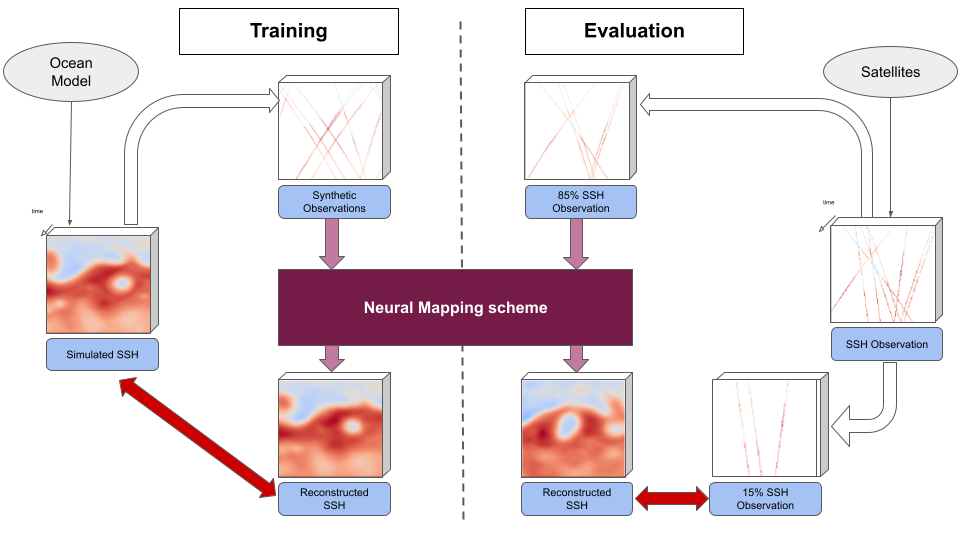
\includegraphics[width=\textwidth]{00_Simulearning/figures/schema_method.png}
    \caption{Overview of the experimental setup. On the left side we display the OSSE training principle based on an ocean simulation which will be used for 1) generating synthetic observation and 2) computing the training objective of the neural mapping scheme. On the right side we show the evaluation principle of splitting the available satellite observations to evaluate the method on data that were not used for the inference.}
    \label{fig:method}
\end{figure}


\subsection{Neural mapping scheme}
\label{ssec:4dvarnet}

We consider the 4DVarNet model for our study. It's a variational data assimilation method where the prior cost formulated using a physically-aware convolutional neural network, and the minimization procedure is done using a recurrent neural network as introduced by \cite{andrychowiczLearningLearnGradient}.
The overall architecture and components are the same as the one described in previous publications \cite{fabletENDTOENDPHYSICSINFORMEDREPRESENTATION2021}. Some changes in the implementation details have been made that were found to empirically improve the performance and reduce the training time. We refer the reader to the code for more details.
This architecture reaches state of the art performance when evaluated in OSSE setup which makes it a good candidate for assessing the generalization to real data


\subsection{SSH Data}
\label{ssec:data}

\begin{table}[h]

\begin{tabular}{ll||cccc}
\toprule
{} & {}& Resolution & Reanalysis & Tide & DAC  \\
\midrule
NATL60 &\cite{ajayiSpatialTemporalVariability2020}               &      1/60 $^\circ$ &               No &            No &                   No  \\
eNATL60-t &\cite{brodeauOceannextENATL60Material2020}         &      1/60 $^\circ$ &               No &           Yes &                  Yes  \\
eNATL60-0 &\cite{brodeauOceannextENATL60Material2020}         &      1/60 $^\circ$ &               No &            No &                  Yes  \\
GLORYS12-r &\cite{jean-michelCopernicusGlobal122021} &      1/12 $^\circ$ &              Yes &            No &                   No  \\
GLORYS12-f &\cite{jean-michelCopernicusGlobal122021}   &      1/12 $^\circ$ &               No &            No &                   No  \\
ORCA025& \cite{bernardImpactPartialSteps2006}             &       1/4 $^\circ$ &               No &            No &                   No  \\
\bottomrule
\end{tabular}
\caption{Summary table of the different synthetic SSH fields used for training}
\label{tab:data}
\end{table}



Digital ocean models are intricate software programs that incorporate numerous configuration parameters. In order to better isolate influence factors, we considered runs of the NEMO\cite{gurvanNEMOOceanEngine2022} ocean model with different configurations. We selected six distinct datasets to examine the influence of three factors on the dynamical structures manifested in the simulations.

In order to evaluate the impact of the grid resolution used for the simulation, we consider the runs NATL60, ORCA025 and the free run of GLORYS12-f  which are respectively run at  1/60°, 1/12°, 1/4°. We know that finer grids allow for more processes to be simulated. We expect dynamics to therefore be closer to the real ocean in higher resolution simulations and the associated trained deep learning model to perform better.
Another way to nudge ocean simulations to more realistic dynamics is by assimilating observation data. To evaluate this aspect we compare the GLORYS12-r reanalysis and its associated the free run GLORYS12-f. Measurements of temperature, sea level, sea ice concentration and salinity have been assimilated during the reanalysis. This comparison will also give indication on the impact of using true observation during the training.
Finally the recent eNATL60 twin simulations  eNATL60-t and eNATL60-0 enable us to evaluate impact of explicit modeling of tide motions.
The characteristics of the different simulation are summarized in Table \ref{tab:data}

\subsection{OSSE training setup}
\label{ssec:training}
The training setup is illustrated on the left part of the Figure \ref{fig:method}.
In order to fairly evaluate the datasets' quality as a training resource, we strive to standardize as many training aspects as possible.
All simulations are regridded to the same resolution (1/20°) and daily averages are used as training target. We generate noise-free pseudo-observations by sampling values of the daily averages corresponding to realistic orbits of a 5 altimeter-constellation. All models are trained using one-year synthetic dataset in a domain around the Gulfstream from (66°W, 32°N) to (54°W, 44°N) in which the same two months are kept for validation. The hyper-parameters of the model and training procedure such as the number of epoch, learning rate scheduler are the same for all the experiments. The models are trained on reconstructing the SSH fields and the amplitude of the gradients as well as a regularization cost on the prior model.

\subsection{OSE evaluation setup}
\label{ssec:eval}
The training setup is illustrated on the right part of the Figure \ref{fig:method}.
The evaluation is done using altimetry data from the constellation of 6 satellites from 2017 (SARAL/Altika, Jason 2, Jason 3, Sentinel 3A, Haiyang-2A and Cryosat-2 ). Five satellites are used as inputs for the mapping and one (Cryosat-2) is kept out for computing the metrics. The metrics are computed in the track geometry on which the gridded product is interpolated on the altimetry tracks. The evaluation domain spans from (65°W, 33°N) to (55°W, 43°N)  and the periods goes from January 1$^{st}$ to December 31$^{st}$ 2017. This setup is standardized in a data-challenge \footnote{https://github.com/ocean-data-challenges/2021a\_SSH\_mapping\_OSE} where various methods have been compared on two metrics. Given $\eta_{c2}$ and $\hat{\eta}$ the measured SSH and the reconstructed SSH respectively; $\mu_{ssh}$ is a score based on the normalized root mean squared (nRMSE) error  computed as $1 - \frac{RMS(\hat{\eta} - \eta_{c2})}{RMS(\eta_{c2})}$ and $\lambda_x$ is the wavelength at which the PSD score  $1 - \frac{PSD(\hat{\eta} - \eta_{c2})}{PSD(\eta_{c2})}$ crosses the $0.5$ threshold, which characterize the scales resolved by the reconstruction (the error below that wavelength is make for more that half of the signal). We reuse these metrics for our study and also consider in Table \ref{tab:res} the root mean square error (RMSE) as well as the nRMSE score of the sea level anomaly $\mu_{sla}$ obtained by subtracting the mean dynamic topography to the SSH. We also assess the performance degradation resulting from the transition from simulated to real data by quantifying the improvement relative to DUACS in scales resolved within OSSE and OSE scenarios.

\section{Results}
\label{sec:results}

\subsection{Benchmarking w.r.t the state of the art}
\label{ssec:benchmarks}

We report in Table \ref{tab:bench} the performance metrics of state of the art approaches ranging from operational observation products, deep learning based mapping schemes trained on observation data as well as methods using explicit integration of a dynamical model.
We compare those methods with the 4DVarNet trained on the eNATL60-0 dataset during this study. 
The OSSE-trained 4DVarNet outperform all other methods on the two metrics considered (22\% improvement in RMSE w.r.t. the DUACS product and 33\% improvement in resolved scales)
We add in this table the GLORYS12 reanalysis metrics which illustrates the challenge of combining large ocean general circulation model and observation data for producing operational observation products.


The last column of the table compares the improvement of $\lambda_x$ with regard to DUACS of the different methods with a simulated setups using the NATL60 simulation in which some of this methods have been evaluated \footnote{https://github.com/ocean-data-challenges/2020a\_SSH\_mapping\_NATL60}. We clearly see how the supervised setting using the full model output as a training target is greatly beneficial to the 4DVarNet in the simulated which achieve an improvement of 47\% twice greater than the second best at 22\%. We can however note that this improvement by 15 point for the OSSE-trained mapping shceme when other methods are significantly more stable. We can deduce that the finer structures that are well reconstructed in the OSSE setup are not as beneficial in the OSE setup. We can attribute this to multiple hypothesis, either they may not be representative of the true ocean, or the real altimetry tracks may limit the ability to reconstruct and/or evaluate them.  



\begin{table}[h]
%\centering
\hspace{-10mm}\begin{tabular}{l||llll|rrrc}
\toprule
 & SSH  & Deep  & Calibrated on  & Physical  & rmse & $\mu_{ssh}$  & $\lambda_x$ & $1 - \frac{\lambda_x}{\lambda_{ref}}$ \\
 &  Only &  Learning &  data from &  Model &  (cm) &  () &  (km) & (\% ose, osse) \\
\midrule
(a) \textbf{4DVarNet} &  Yes & Yes & Simulation  & -- & \textbf{5.9}  & \textbf{0.91}  & \textbf{100} & \textbf{33}, \textbf{47} \\
(b) MUSTI & No &  Yes & Satellite  & -- & 6.3  & 0.90  & 112 & 26, 22 \\
(c) ConvLstm-SST & No &  Yes & Satellite  & -- & 6.7  & 0.90  & 108 & 28, -- \\
(d) ConvLstm &  Yes &  Yes & Satellite  & -- & 7.2  & 0.89  & 113 & 25, -- \\
(e) DYMOST&  Yes & No & Satellite  & QG & 6.7  & 0.90  & 131 & 13, 11 \\
(f) MIOST &  Yes & No & Satellite  & -- & 6.8  & 0.90  & 135 & 11, 10 \\
(g) BFN-QG &  Yes & No & Satellite  & QG & 7.6  & 0.89  & 122 & 19, 21 \\
(h) DUACS &  Yes & No & Satellite  & -- & 7.7  & 0.88  & 151 &  ~0,  0 \\
(i) GLORYS12 & No & No & Satellite  & NEMO & 15.1  & 0.77  & 241 & -60, -- \\
\bottomrule
\end{tabular}
\caption{ Benchmark of different methods on the SSH reconstruction of Gulfstream domain: (a) 4dVarNet trained on eNATL60-0 (b) \cite{archambaultMultimodalUnsupervisedSpatioTemporal2023}, (c and d) \cite{martinSynthesizingSeaSurface2023}, (e) \cite{ballarottaDynamicMappingAlongTrack2020}, (f) \cite{ubelmannReconstructingOceanSurface2021}, (g) \cite{guillouMappingAltimetryForthcoming2021}, (h) \cite{taburetDUACSDT2018252019}, (i) \cite{jean-michelCopernicusGlobal122021}. The columns indicate in order: whether ancillary data other than altimetry tracks were used for the mapping (for example sea surface temperature observation products); if the method uses deep learning architectures; the data used to calibrate (or train) the method parameters; the numerical model of the ocean used for the mapping if any (QG stands for quasi-geostrophic); $\mu$ and $\lambda_x$ are the metrics as described in \ref{ssec:eval}}
\label{tab:bench}
\end{table}



\begin{figure}[H]
\begin{minipage}{.80\linewidth}
\begin{subfigure}[t]{.9\linewidth}
\small
\begin{center}
\setlength{\tabcolsep}{1pt}

\begin{tabular}[t]{c@{}cccccc}

\hspace{0cm} ORCA025 & 
 GLORYS12-f & 
 GLORYS12-r & 
 NATL60 & 
 eNATL60-t & 
 eNATL60-0 & \\

%\vspace{-2mm}
%%%%% ORCA025 %%%%%%%%

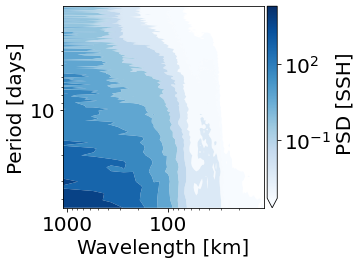
\includegraphics[trim={0 19mm 35mm 5mm},clip, width=2.3cm,height=2cm]{00_Simulearning/figures/plots2/orca025_train_psd_spacetime.png} &
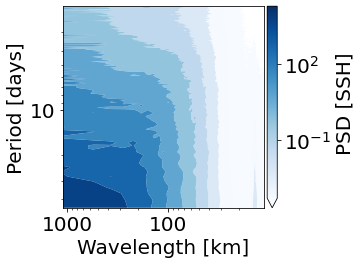
\includegraphics[trim={19mm 19mm 35mm 5mm},clip, width=2cm,height=2cm]{00_Simulearning/figures/plots2/glorys12-f_train_psd_spacetime.png} &
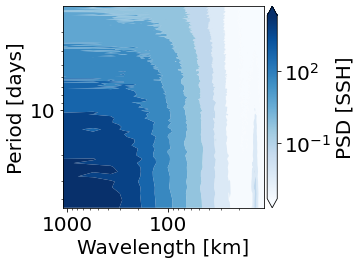
\includegraphics[trim={19mm 19mm 35mm 5mm},clip, width=2cm,height=2cm]{00_Simulearning/figures/plots2/glorys12-r_train_psd_spacetime.png} &
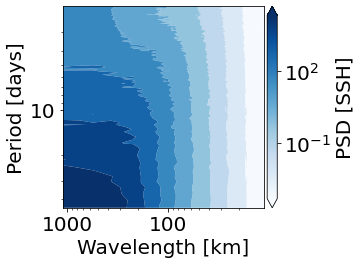
\includegraphics[trim={19mm 19mm 35mm 5mm},clip, width=2cm,height=2cm]{00_Simulearning/figures/plots2/natl60_train_psd_spacetime.png} &
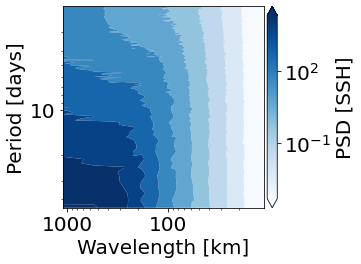
\includegraphics[trim={19mm 19mm 35mm 5mm},clip, width=2cm,height=2cm]{00_Simulearning/figures/plots2/enatl60-t_train_psd_spacetime.png} &
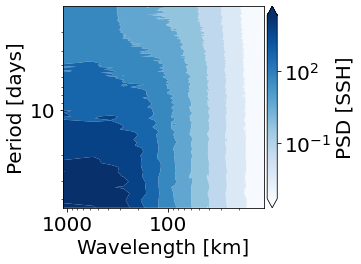
\includegraphics[trim={19mm 19mm 35mm 5mm},clip, width=2cm,height=2cm]{00_Simulearning/figures/plots2/enatl60-0_train_psd_spacetime.png} &
 \\
%\vspace{3mm}
%%%%% GLORYS12-f %%%%%%%%

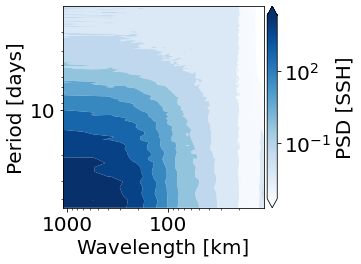
\includegraphics[trim={0mm 0 35mm 5mm},clip, width=2.3cm,height=2.3cm]{00_Simulearning/figures/plots2/orca025_rec_psd_spacetime.png} &
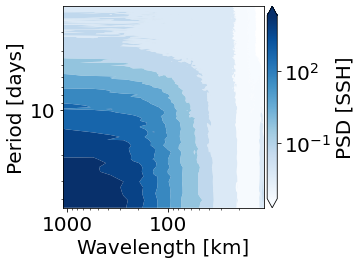
\includegraphics[trim={19mm 0 35mm 5mm},clip, width=2cm,height=2.3cm]{00_Simulearning/figures/plots2/glorys12-f_rec_psd_spacetime.png} &
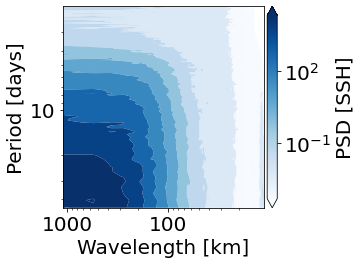
\includegraphics[trim={19mm 0 35mm 5mm},clip, width=2cm,height=2.3cm]{00_Simulearning/figures/plots2/glorys12-r_rec_psd_spacetime.png}&
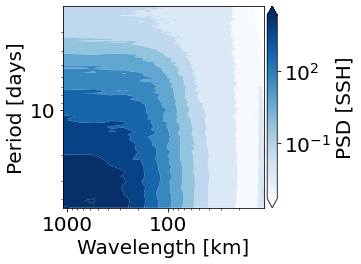
\includegraphics[trim={19mm 0 35mm 5mm},clip, width=2cm,height=2.3cm]{00_Simulearning/figures/plots2/natl60_rec_psd_spacetime.png}&
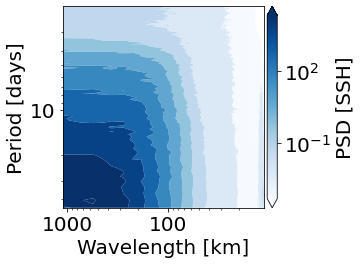
\includegraphics[trim={19mm 0 35mm 5mm},clip, width=2cm,height=2.3cm]{00_Simulearning/figures/plots2/enatl60-t_rec_psd_spacetime.png} &
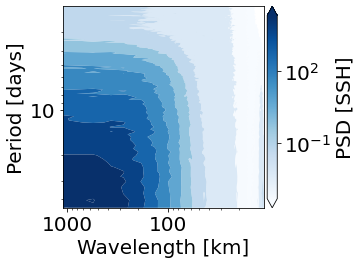
\includegraphics[trim={19mm 0 35mm 5mm},clip, width=2cm,height=2.3cm]{00_Simulearning/figures/plots2/enatl60-0_rec_psd_spacetime.png}  &
\\

\end{tabular}
% \caption{Row I - Isotrophic PSD. Row 2 - Isotrophic PSD Score}

\end{center}

\end{subfigure}
\end{minipage}
\hspace{1.5cm}\begin{minipage}{0.01\linewidth}
\vspace{-.5cm}

\begin{subfigure}[t]{.9\linewidth}
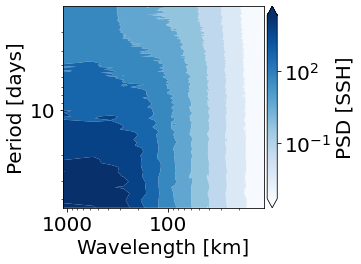
\includegraphics[trim={9.4cm 0 0 0},clip, width=0.88cm,height=2.52cm]{00_Simulearning/figures/plots2/enatl60-0_train_psd_spacetime.png}
\end{subfigure}
\end{minipage}
\caption{
Space-time spectral densities of the training datasets (first row) and their associated reconstructions (second row). We see how finer resolution and reanalysis increase the energy levels at all scales in the while the reconstructions' PSDs are more alike but with still visible differences especially in the temporal axis} \vspace{-5mm}
\label{fig:spacetime_psd}
\end{figure}




\begin{figure}[H]
\small
\begin{center}
\setlength{\tabcolsep}{1pt}
\begin{tabular}{ccccc}
 &&
&\hspace{-30mm} 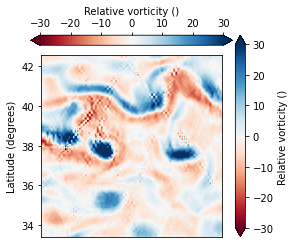
\includegraphics[trim={8mm 7cm 22mm 0},clip,width=3.0cm,height=0.7cm]{00_Simulearning/figures/plots/horizontal_cbar_vort.png} &\\
\hspace{0mm} &&
\hspace{-30mm} Training  
\hspace{3mm}  & 
 & 
\hspace{-30mm} Reconstruction \\

%\vspace{-2mm}
%%%%% ORCA025 %%%%%%%%

\hspace{-10mm}  1)&
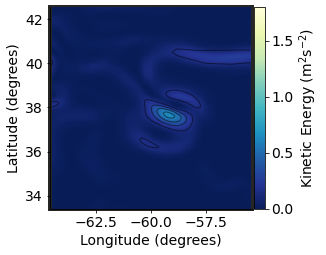
\includegraphics[trim={0 16mm 26mm 5mm},clip, width=3.3cm,height=2.9cm]{00_Simulearning/figures/plots2/orca025_train_ke.png} &
 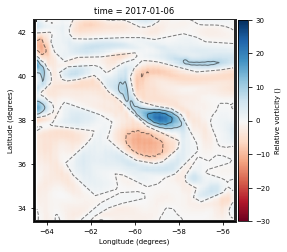
\includegraphics[trim={13mm 13mm 22mm 6mm},clip, width=2.9cm,height=2.9cm]{00_Simulearning/figures/plots/orca025_train_vort_r.png} &
 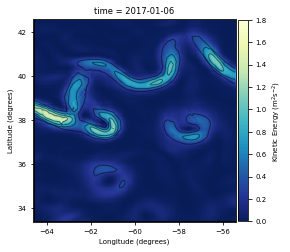
\includegraphics[trim={13mm 13mm 22mm 6mm},clip, width=2.9cm,height=2.9cm]{00_Simulearning/figures/plots/orca025_rec_ke.png} &
 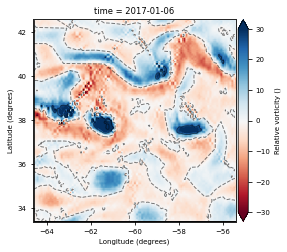
\includegraphics[trim={13mm 13mm 22mm 6mm},clip,width=2.9cm,height=2.9cm]{00_Simulearning/figures/plots/orca025_rec_vort_r.png} \\
%\vspace{3mm}
%%%%% GLORYS12-f %%%%%%%%
\hspace{-10mm} 2) &
 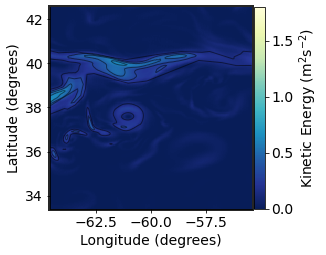
\includegraphics[trim={0 16mm 26mm 5mm},clip, width=3.3cm,height=2.9cm]{00_Simulearning/figures/plots2/glorys12-f_train_ke.png} &
 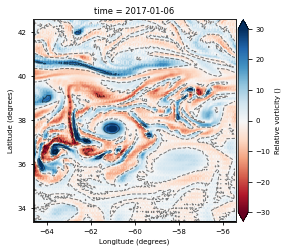
\includegraphics[trim={13mm 13mm 22mm 6mm},clip, width=2.9cm,height=2.9cm]{00_Simulearning/figures/plots/glorys12-f_train_vort_r.png} &
 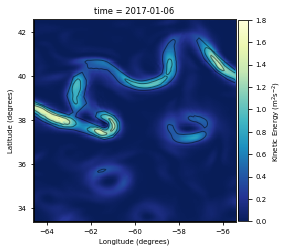
\includegraphics[trim={13mm 13mm 22mm 6mm},clip, width=2.9cm,height=2.9cm]{00_Simulearning/figures/plots/glorys12-f_rec_ke.png} &
 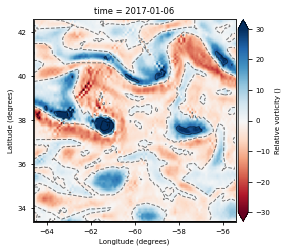
\includegraphics[trim={13mm 13mm 22mm 6mm},clip,width=2.9cm,height=2.9cm]{00_Simulearning/figures/plots/glorys12-f_rec_vort_r.png} \\
%\vspace{3mm}
%%%%% GLORYS12-f %%%%%%%%
\hspace{-10mm} 3) &
 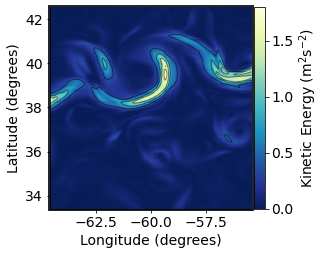
\includegraphics[trim={0 16mm 26mm 5mm},clip, width=3.3cm,height=2.9cm]{00_Simulearning/figures/plots2/glorys12-r_train_ke.png} &
 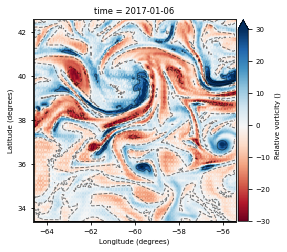
\includegraphics[trim={13mm 13mm 22mm 6mm},clip, width=2.9cm,height=2.9cm]{00_Simulearning/figures/plots/glorys12-r_train_vort_r.png} &
 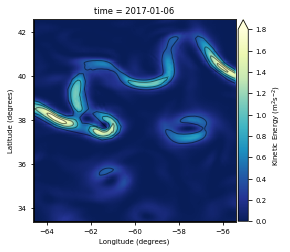
\includegraphics[trim={13mm 13mm 22mm 6mm},clip, width=2.9cm,height=2.9cm]{00_Simulearning/figures/plots/glorys12-r_rec_ke.png} &
 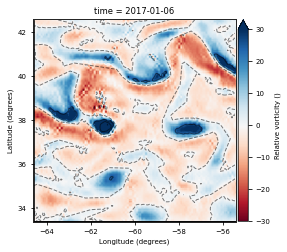
\includegraphics[trim={13mm 13mm 22mm 6mm},clip,width=2.9cm,height=2.9cm]{00_Simulearning/figures/plots/glorys12-r_rec_vort_r.png} \\
%%%%% NATL60 %%%%%%%%
\hspace{-10mm} 4) &
 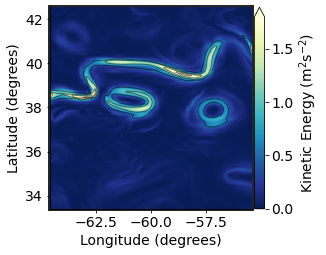
\includegraphics[trim={0 16mm 26mm 5mm},clip, width=3.3cm,height=2.9cm]{00_Simulearning/figures/plots2/natl60_train_ke.png} &
 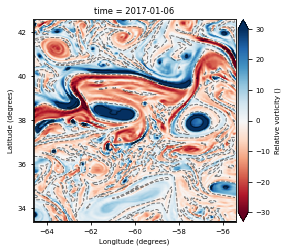
\includegraphics[trim={13mm 13mm 22mm 6mm},clip, width=2.9cm,height=2.9cm]{00_Simulearning/figures/plots/natl60_train_vort_r.png} &
 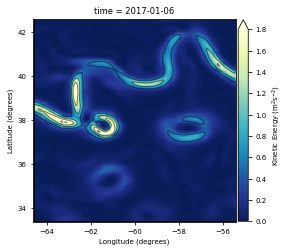
\includegraphics[trim={13mm 13mm 22mm 6mm},clip, width=2.9cm,height=2.9cm]{00_Simulearning/figures/plots/natl60_rec_ke.png} &
 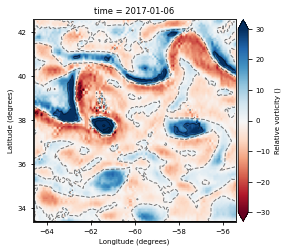
\includegraphics[trim={13mm 13mm 22mm 6mm},clip,width=2.9cm,height=2.9cm]{00_Simulearning/figures/plots/natl60_rec_vort_r.png} \\
%\vspace{3mm}
%%%%% eNATL60-t %%%%%%%%
\hspace{-10mm} 5) &
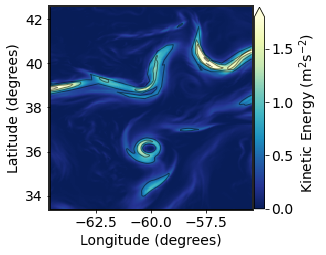
\includegraphics[trim={0 16mm 26mm 5mm},clip, width=3.3cm,height=2.9cm]{00_Simulearning/figures/plots2/enatl60-t_train_ke.png} &
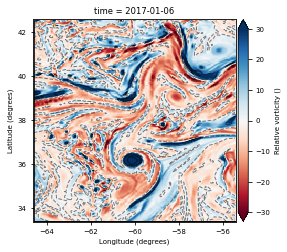
\includegraphics[trim={13mm 13mm 22mm 6mm},clip, width=2.9cm,height=2.9cm]{00_Simulearning/figures/plots/enatl60-t_train_vort_r.png} &
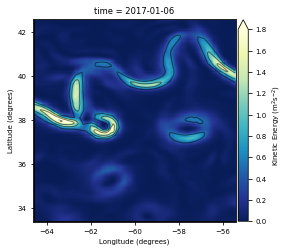
\includegraphics[trim={13mm 13mm 22mm 6mm},clip, width=2.9cm,height=2.9cm]{00_Simulearning/figures/plots/enatl60-t_rec_ke.png} &
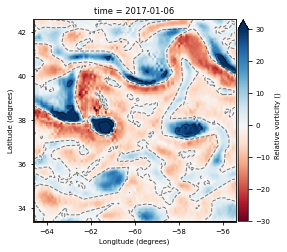
\includegraphics[trim={13mm 13mm 22mm 6mm},clip,width=2.9cm,height=2.9cm]{00_Simulearning/figures/plots/enatl60-t_rec_vort_r.png} \\
%\vspace{3mm}
%%%%% eNATL60-0 %%%%%%%%
% \hspace{-10mm} 6) &
%  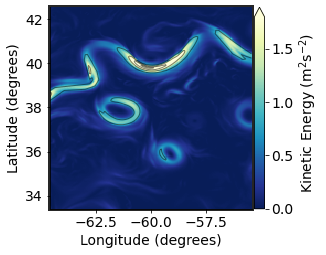
\includegraphics[trim={0 0 19mm 5mm},clip, width=3.3cm,height=3.1cm]{00_Simulearning/figures/plots2/enatl60-0_train_ke.png} &
%  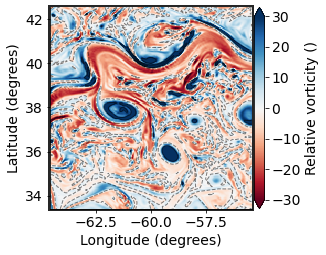
\includegraphics[trim={13mm 0 22mm 5mm},clip, width=2.9cm,height=3.1cm]{00_Simulearning/figures/plots2/enatl60-0_train_vort_r.png} &
%  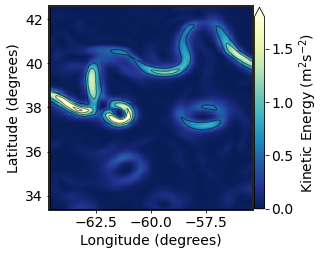
\includegraphics[trim={13mm 0 22mm 5mm},clip, width=2.9cm,height=3.1cm]{00_Simulearning/figures/plots2/enatl60-0_rec_ke.png} &
%  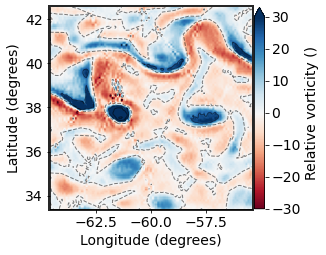
\includegraphics[trim={13mm 0 22mm 5mm},clip,width=2.9cm,height=3.1cm]{00_Simulearning/figures/plots2/enatl60-0_rec_vort_r.png} \\
 \hspace{-10mm} 6) &
 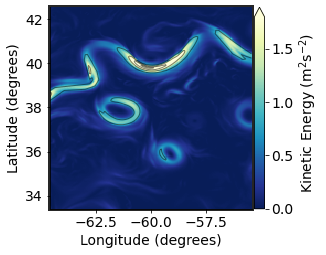
\includegraphics[trim={0 0 25mm 5mm},clip, width=3.3cm,height=3.1cm]{00_Simulearning/figures/plots2/enatl60-0_train_ke.png} &
 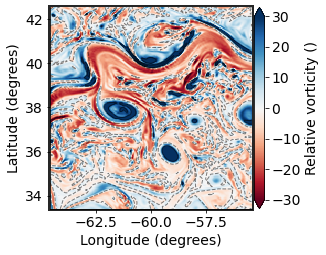
\includegraphics[trim={18mm 0 26mm 5mm},clip, width=2.9cm,height=3.1cm]{00_Simulearning/figures/plots2/enatl60-0_train_vort_r.png} &
 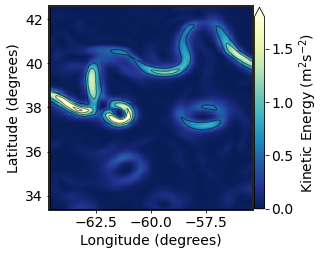
\includegraphics[trim={18mm 0 26mm 5mm},clip, width=2.9cm,height=3.1cm]{00_Simulearning/figures/plots2/enatl60-0_rec_ke.png} &
 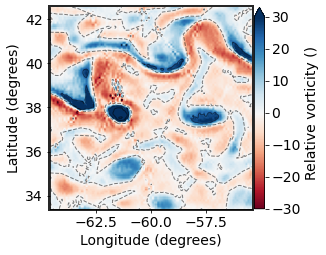
\includegraphics[trim={18mm 0 26mm 5mm},clip,width=2.9cm,height=3.1cm]{00_Simulearning/figures/plots2/enatl60-0_rec_vort_r.png} \\
 \hspace{-15mm} &(a) & (b) & (c) & (d) \\
 &&
&\hspace{-30mm} 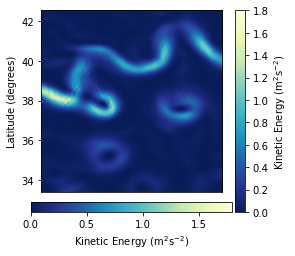
\includegraphics[trim={8mm 0 22mm 7cm},clip,width=2.5cm,height=0.7cm]{00_Simulearning/figures/plots/horizontal_cbar_ke_bottom.png} &\\
% \vspace{-2mm}

\end{tabular}
\vspace{-3mm}
% \caption{Row I - Isotrophic PSD. Row 2 - Isotrophic PSD Score}
\caption{
Kinetic energy ((a) and (c) and relative vorticity ((b) and (d)) of the training dataset ((a) and (b)) and the associated 4DVarNet reconstructions ((c) and (d)) at the 6$^th$ of January of their respective year.
Each row shows the experiment using: 1) ORCA025, 2) GLORYS12-f, 3) GLORYS12-r, 4) NATL60, 5) eNATL60-t, 6) eNATL60-0}
\vspace{-5mm}
\label{fig:maps}
\end{center}
\end{figure}



\begin{table}[H]
\centering
\begin{tabular}{l||rrrrc}
\toprule
Training Data & RMSE  & $\mu_{ssh}$  & $\mu_{sla}$ & $\lambda_x$ & $1 - \frac{\lambda_x}{\lambda_{ref}}$ \\
 &  (cm) &  () &  () &  (km) & (\% ose, osse) \\
\midrule
NATL60 & \textbf{5.9}  & \textbf{0.91}  & \textbf{0.80}  & \textbf{98} & (\textbf{35}, --)\\
eNATL60-t & \textbf{5.9}  & \textbf{0.91}  & \textbf{0.80}  & 100 & (33, \textbf{48})\\
eNATL60-0 & \textbf{5.9}  & \textbf{0.91}  & \textbf{0.80}  & 100 & (33, 47)\\
GLORYS12-r & 6.3  & 0.90  & 0.78  & 106  & (30, 28)\\
GLORYS12-f & 6.7  & 0.90  & 0.77  & 119 & (21, 23)\\
ORCA025 & 7.1  & 0.89  & 0.76  & 126 & (17, 17)\\
\bottomrule
\end{tabular}

\caption{Performance comparison of 4dVarNet mapping schemes trained on different simulated datasets. The first column show the source of the training dataset as described in Table \ref{tab:data}. The subsequent columns indicate the reconstruction metrics described in Section \ref{ssec:eval}. Note that the NATL60 could not be evaluated on the OSSE setup since the evaluation data were used for validation during the training stage.}
\label{tab:res}
\end{table}

\subsection{Eddy-permitting vs eddy-resolving simulations}
\label{ssec:resolution}


\begin{figure}[H]
\small
\setlength{\tabcolsep}{1pt}
\begin{tabular}{ccc}

\hspace{3mm} Training PSD & 
\hspace{3mm} Reconstruction PSD & 
\hspace{3mm} PSD Score  \\

%\vspace{-2mm}
%%%%% ORCA025 %%%%%%%%

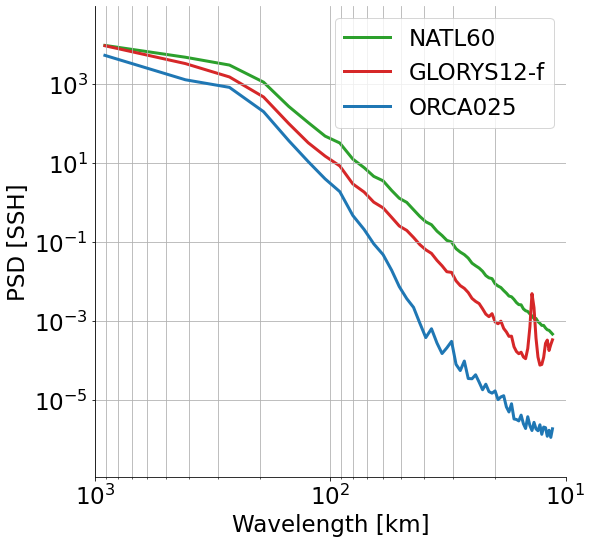
\includegraphics[width=0.31\textwidth]{00_Simulearning/figures/plots2/isotrop_psd_res_train.png} &
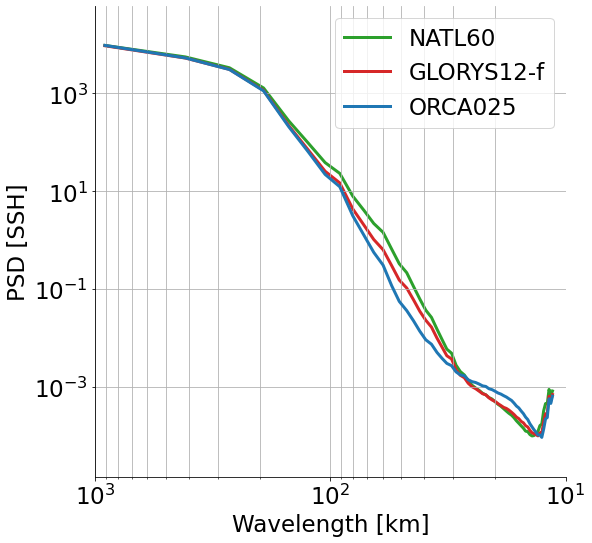
\includegraphics[width=0.31\textwidth]{00_Simulearning/figures/plots2/isotrop_psd_res_rec.png} &
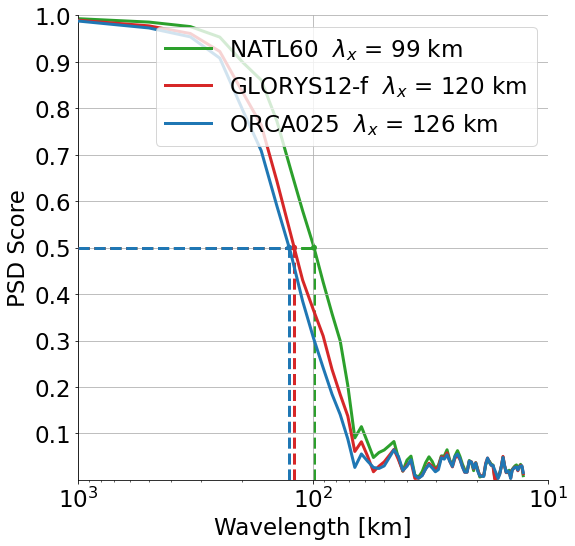
\includegraphics[width=0.31\textwidth]{00_Simulearning/figures/plots2/res_1d_psd_score.png}


\end{tabular}
\vspace{-3mm}
% \caption{Row I - Isotrophic PSD. Row 2 - Isotrophic PSD Score}
\caption{
Impact of the resolution on the PSDs. We display the PSD of the training dataset (left plot), reconstructed SSH field (center plot) as well as the associated PSD score (right plot)}\vspace{-5mm}
\label{fig:respsd}
\end{figure}


We analyse here in more detail the impact of ocean run resolution in the training data and reconstructed fields. Looking at quantitative metrics in Table \ref{tab:res} we see the expected trend that using a higher resolution grid in the ocean run simulation enables a better outcome with a 22\% improvement in scales resolved and 17\% improvement in RMSE between the experiments with the coarsest (ORCA025) and finest (NATL60) resolution.
Qualitative differences can also been seen in the relative vorticity fields in Figure \ref{fig:maps} where residual artifacts due to the altimetry tracks can be seen (60°W, 39°N) for the two lower resolution training and are greatly diminished when looking at the NATL60 resolution. 
However we see that the reconstructed vorticity and kinetic energy of the ORCA025 experiment are quite similar to the one from the NATL60 experiment despite the ORCA025 training data clearly containing fewer fine scale structures an weaker gradients. The trained model is able to reconstruct fields outside the training distribution when prompted with observations different from the training data. 

This is also visible in the spectral densities shown in Figure \ref{fig:respsd} where we see that the gap in energy distribution of the training data has been significantly reduced in the reconstructions, however the PSD score plot on the right shows that even if the energy levels are close in the reconstructions, training with finer resolution produces a more faithful reconstruction at all scales.
Finally when looking at the space-time PSD in Figure \ref{fig:spacetime_psd}, we can note that even though the spatial spectra have been greatly homogenized, the temporal PSD still contains significant gaps of an order of magnitude for periods greater than 10 days and wavelength greater than 200km.

\subsection{Impact of reanalysis datasets}
\label{ssec:reanalysis}
\begin{figure}[h]

\small

\setlength{\tabcolsep}{1pt}
\begin{tabular}{ccc}

\hspace{3mm} Training PSD & 
\hspace{3mm} Reconstruction PSD & 
\hspace{3mm} PSD Score  \\

%\vspace{-2mm}
%%%%% ORCA025 %%%%%%%%

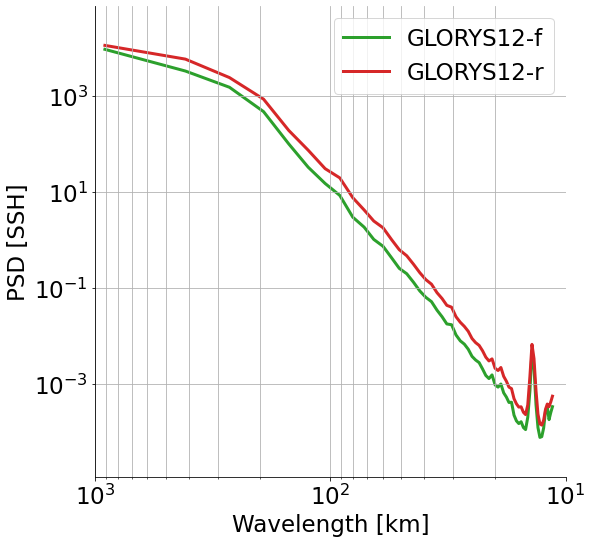
\includegraphics[width=0.31\textwidth]{00_Simulearning/figures/plots2/isotrop_psd_rea_train.png} &
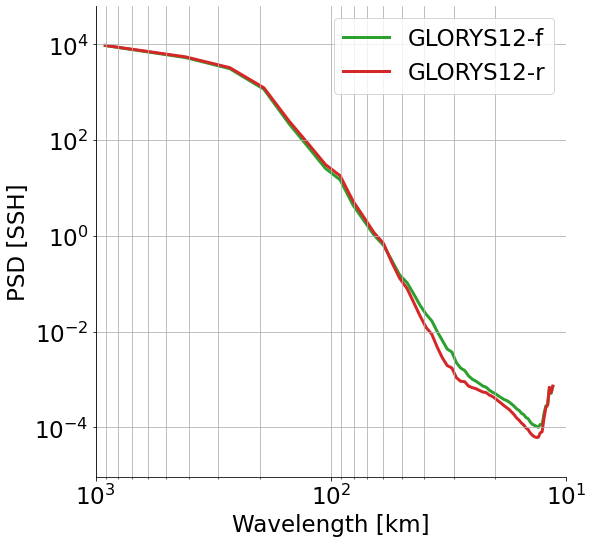
\includegraphics[width=0.31\textwidth]{00_Simulearning/figures/plots2/isotrop_psd_rea_rec.png} &
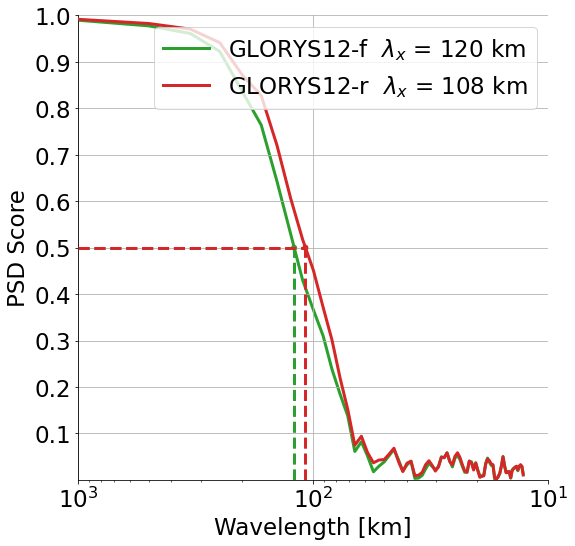
\includegraphics[width=0.31\textwidth]{00_Simulearning/figures/plots2/rea_1d_psd_score.png}


\end{tabular}
\vspace{-3mm}
% \caption{Row I - Isotrophic PSD. Row 2 - Isotrophic PSD Score}
\caption{
Impact of model reanalysis on the PSDs. We display the PSD of the training dataset (left plot), reconstructed SSH field (center plot) as well as the associated PSD score (right plot)}\vspace{-5mm}
\label{fig:reapsd}

\end{figure}

Looking in more specifically at the effect of ocean reanalysis between the two experiments GLORYS12-f and GLORYS12-r. We can first note the impact of observation data assimilation in Figure \ref{fig:spacetime_psd} where we see how the power spectrum of the reanalysis is significantly raised compared to the free run and is similar the one of the finer resolution simulation. Visually on the maps in Figure \ref{fig:maps}, we can also clearly see stronger gradients in the kinetic energy.

We can observe a similar behavion as in section \ref{ssec:resolution} in Figure \ref{fig:reapsd} with the gap of in spectral density being diminished between the training and reconstruction data, and the PSD score indicating a lower energy of the error at all scales for the reanalyzed experiment.

Quantitatively in Table \ref{tab:data} we see an improvement of 11\% in both the RMSE and the scale resolved, and one singular fact is that training on a reanalysis increase the relative gain w.r.t. DUACS significantly more on real data (+9\%) than on simulated data (+5\%) as we can right most column. This can be explained thanks to the fact the training data integrates information from real world observations which reduces the generalization problem to real altimetry mapping.

\subsection{Impact of tide-resolving numerical simulations}
\label{ssec:tide}
\begin{figure}[H]
\small
\begin{center}
\setlength{\tabcolsep}{1pt}
\begin{tabular}{ccc}

\hspace{3mm} Training PSD & 
\hspace{3mm} Reconstruction PSD & 
\hspace{3mm} PSD Score  \\

%\vspace{-2mm}
%%%%% Tide psd %%%%%%%%

\includegraphics[width=0.31\textwidth]{00_Simulearning/figures/plots2/isotrop_psd_tide_train.png} &
\includegraphics[width=0.31\textwidth]{00_Simulearning/figures/plots2/isotrop_psd_tide_rec.png} &
\includegraphics[width=0.31\textwidth]{00_Simulearning/figures/plots2/tide_1d_psd_score.png}


\end{tabular}
\vspace{-3mm}
% \caption{Row I - Isotrophic PSD. Row 2 - Isotrophic PSD Score}
\caption{
Impact of explicit tide modelling on the PSDs. We display the PSD of the training dataset after the prepocessing (left plot), the reconstructed SSH field (center plot) as well as the associated PSD score (right plot)}\vspace{-5mm}
\label{fig:tidepsd}
\end{center}
\end{figure}

We compare here the effect of explicit tide modeling in the training simulation. For this we use the twin eNATL60 simulation runs eNATL60-t and eNATL60-0.  Contrary to other runs, those simulation contains barometric and wind forcing, we therefore remove the Dynamic Atmospheric Correction from the SSH fields. Additionally since the barotropic tides signal are removed from real altimetry tracks prior to interpolation, we also remove this signal from the training data by subtracting the spatial mean over the training domain for each hourly snapshot before calculating the daily averages.  

After those processing steps, we see that the two training datasets contain very similar spectral profiles as shown in Figures \ref{fig:spacetime_psd} and \ref{fig:tidepsd}. 
We also find that training on those two dataset produce little differences in the reconstructions both quantitatively \ref{tab:bench} and qualitatively (Fig. \ref{fig:maps}) and both experiments' results are comparable to the NATL60 experiment.
 
We identify two hypothesis linked to the lack of impact of resolving tides during the simulation:
\begin{itemize}
    \item The preprocessing applied on the training field remove the main tide signals. We therefore effectively measure the impact of tide modeling on other ocean processes that may be less significant.
    \item The evaluation procedure applied on altimetry tracks on which the barotropic tide has been filtered may not be interpretable enough to measure the reconstruction of residual tide signals. New instruments like the KaRIN deployed in the SWOT mission may provide new ways to better quantify those effects.   
\end{itemize}

These findings provide motivation for carefully considering the purpose of the learning-based model when making decisions about the training data. Indeed In our case, explicitly modeling tide processes that are removed from the observations in the evaluation setup added overhead in the computational cost of running the simulation as well as in the preprocessing of the training data. Additionally given the considered evaluation data and metrics, we were not able to quantify any significant differences between the two trained mapping schemes.

On the other hand training on a simulation with tide could also be a way to reduce the processing steps on the observation data by being able to interpolate observation containing the tide signals.

\section{Discussion}
\label{sec:discussion}
This study has been greatly facilitated by the standardized tasks and evaluation setups proposed in data-challenges \footnote{https://ocean-data-challenges.github.io/}. The specification of problems by domain experts through datasets and relevant evaluation metrics have been instrumental in constituting the comprehensive benchmark combining methods from different teams and institution around the world. Additionally, it also constitutes a strong basis for multi-disciplinary collaboration between the ocean and machine learning research communities.

Moreover, the results presented in this study introduce a direct relation between ocean simulations and the performance of altimetry products. This opens new ways for ocean physicist, modelers and operational oceanographers to collaborate. In order to assess the range of these new synergies, it would be interesting to explore if the approach proposed here of training altimetry mapping schemes using simulation data would generalize to other tasks such as forecast or sensor calibration and to other quantities like surface temperature, currents, salinity or biochemical tracers.

If the approach turns out generic enough, one could envision training large foundation deep learning models capturing the inner structure of high resolution ocean simulations which could then be used in many downstream applications. This could be the way to capitalize on all the advancement in ocean modeling without having to run OGCM numerical simulation for each downstream products.    

As a final point we would like to highlight the cost consideration when running numerical simulation intended for training learning based schemes. Indeed given that the eNATL60 run took 2700x CPU hours and 350x memory compared to the ORCA025 run for a smaller domain, a trade-off arises between generating multiple "cheap" trajectories versus generating  a single more realistic trajectory. 

\section{Conclusion}
\label{sec:conclusion}
We've seen in this study that training machine learning models on simulations offers reliably good performance on real altimetry data mapping and outperforms current state of the art approaches. Even the coarsest simulation considered ORCA025 provides competitive results with current operational methods. We have shown that using a more realistic SSH fields using reanalysis or higher resolution simumlations increases the performances of the trained model. This is an exciting result that shows the potential for training operational products from ocean simulations and how advances in ocean modeling in operational oceanography can be beneficial. The results shown here are limited to the interpolation problem on a regional domain but the robustness of the performance shown are encouraging for further developing these results using a bigger domain.


\addcontentsline{toc}{section}{Bibliography}
\putbib[./00_Simulearning/biblio]
\end{bibunit}
% \bibliography{biblio}

% \section*{Open Research Section}
% The authors provide the training data, source code, reconstructed maps and trained model for each experiments of the manuscript through the following link https://doi.org/10.5281/zenodo.8064114.



% \acknowledgments
% This work was supported by ANR Projects Melody and OceaniX and CNES. It benefited from HPC and GPU resources from GENCI-IDRIS (Grant 2020-101030) and Ifremer.


% \bibliography{biblio}



% \end{document}






